\problemname{Carrots}
\noindent
Tor and his mother love carrots.
Every day, they place a bowl with 40 carrots and then eat carrots continuously until the bowl is empty.
If they are both ready to take a carrot when there is only one left, neither of them will take the last one.

\begin{figure}[h]
    \centering
  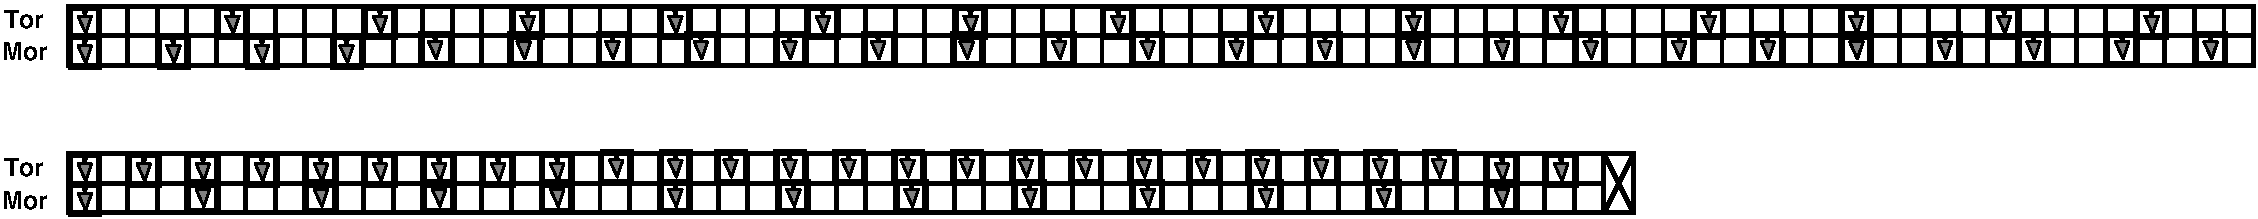
\includegraphics[width=1.0\textwidth]{morot.pdf}
  \caption{Timetable for carrot eating in example 1 (top) and example 2 (bottom). In the second example,
  no one will take the last carrot.}
\end{figure}

Write a program that, given the number of seconds it takes for Tor and his mother to eat each carrot (both integers),
calculates how many carrots each of them gets.

\section*{Input}
The first and only line input contains the integers $T$ and $M$ ($1 \leq T, M \leq 100$), the time it takes for Tor and
his mother respectively to eat a carrot, in seconds.

\section*{Output}
Print two integers: first the number of carrots that Tor eats, followed by the number of carrots his mother eats.

\section*{Points}
Your solution will be tested on several test case groups.
To get the points for a group, it must pass all the test cases in the group.

\noindent
\begin{tabular}{| l | l | p{12cm} |}
  \hline
  \textbf{Group} & \textbf{Point value} & \textbf{Constraints} \\ \hline
  $1$    & $40$      & Tor and his mother are never ready to eat a carrot at the same time after having eaten their first carrots. \\ \hline
  $2$    & $60$      & No additional constraints. \\ \hline
\end{tabular}
